\documentclass{article}
\usepackage[utf8]{inputenc}
\usepackage{enumerate}
\usepackage{amsmath}
\usepackage{amssymb}
\usepackage{amsfonts}
\usepackage{amstext}
\usepackage{amsthm}
\usepackage{mathtools}
\usepackage{tikz}
\usepackage{tikz-3dplot}
\usetikzlibrary{angles, quotes}
\usepackage{amssymb}
\usepackage{amsmath}
\usepackage{cancel}
\DeclarePairedDelimiter{\ceil}{\lceil}{\rceil}
\title{Calculus III Review Sheet 1 Practice}
\author{Eddie Ozuna,Tyler Franklin}

\begin{document}
\maketitle
\begin{enumerate}[1.]
\item\textbf{Prove that for any two vectors u and v, the inner product of u and v is equal to $\mid\vec{u}\mid\mid\vec{v}\mid\cos(\theta)$ where $\theta$ is the angle between $\vec{u}$ and $\vec{v}$.\\\\Hint: Draw the picture and recall the Law of Cosines is just a degeneration of
the Pythagorean Theorem:}\\
\\
Derivation: Law of Cosine\\
	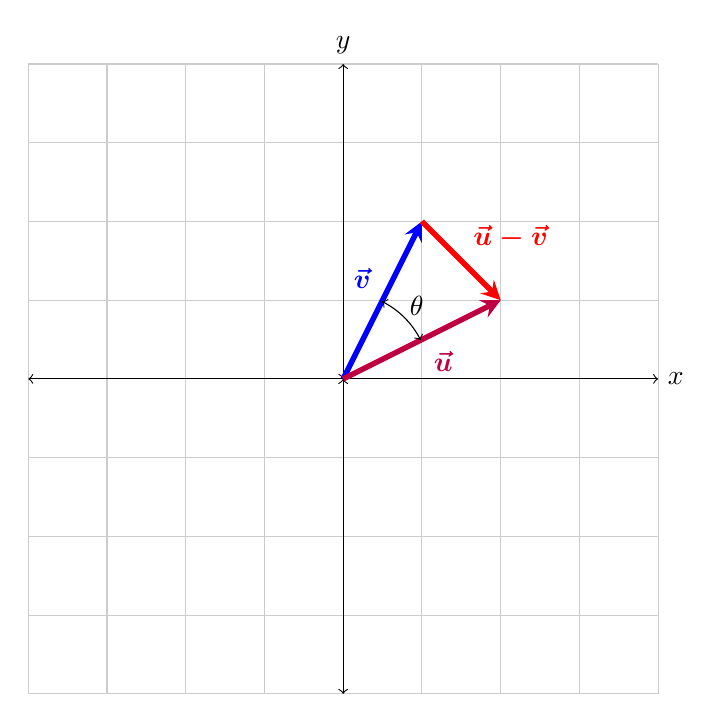
\begin{tikzpicture}
  \draw[thin,gray!40] (-4,-4) coordinate (o) grid (4,4);
  \draw[<->] (0,0)--(0,0) coordinate (o) node[right]{};
  \draw[<->] (-4,0)--(4,0)  node[right]{$x$};
  \draw[<->] (0,-4)--(0,4)  node[above]{$y$};
  \draw[line width=2pt,blue,-stealth](0,0)--(1,2) coordinate (x) node[midway,auto]{$\boldsymbol{\vec{v}}$};
  \draw[line width=2pt,purple,-stealth](0,0)--(2,1) coordinate (y) node[midway,auto,swap]{$\boldsymbol{\vec{u}}$};
  \draw[line width=2pt,red,-stealth](1,2)--(2,1) node[midway,auto]{$\boldsymbol{\vec{u}-\vec{v}}$};
 \pic [draw, <->,
      angle radius=11mm, angle eccentricity=1.2,
      "$\theta$"] {angle = y--o--x};
\end{tikzpicture}\\
$\mid\vec{u}-\vec{v}\mid^{2} = \mid\vec{u}\mid^{2} + \mid\vec{v}\mid^{2}-\hspace{.1cm}2\mid\vec{u}\mid\cdot\mid\vec{v}\mid\cos(\theta)$\\
\\
$\cancel{\mid\vec{u}\mid^{2}}-\hspace{.1cm}2\vec{v}\cdot\vec{u}\hspace{.1cm}+\cancel{\mid\vec{v}\mid^{2}}=\cancel{\mid\vec{u}\mid^{2}} + \cancel{\mid\vec{v}\mid^{2}}-2\mid\vec{u}\mid\cdot\mid\vec{v}\mid\cos(\theta)$\\
\\
$\cancel{-2}\vec{v}\cdot\vec{u} = \cancel{-2}\mid\vec{u}\mid\cdot\mid\vec{v}\mid\cos(\theta)$\\
\\
$\vec{v}\cdot\vec{u} = \mid\vec{u}\mid\cdot\mid\vec{v}\mid\cos(\theta)$\\
\end{enumerate}
\begin{enumerate}[2.]
\item\textbf{Are the vectors $\vec{u}=\left(\!\begin{array}{c}1 \\ 2 \\  3\end{array} \!\right)$ , $\vec{v}=\left(\!\begin{array}{c}-2 \\ 1 \\  0\end{array} \!\right)$ orthogonal? Why or why not?}\\
\\
Vectors are orthogonal(perpendicular) if and only if the result of the dot product is zero.\\
\\
($\vec{u}\cdot\vec{v})=(1\cdot-2)+(2\cdot1)+(3\cdot0)=0$
\\
\\
Yes they are orthogonal 
\end{enumerate}
\begin{enumerate}[3]
\item\textbf{Prove that the cross product of two vectors $\vec{u}$ and $\vec{v}$ is actually orthogonal to each of $\vec{u}$ and $\vec{v}$ simultaneously, i.e. $\vec{u}\times\vec{v}$ is orthogonal to $\vec{u}$ and $\vec{u}\times\vec{v}$ is
orthogonal to $\vec{v}$ }
\\
\\
Step 1. Take the cross product of $\vec{u}$ and $\vec{v}$\\
\\
$\vec{u}\times\vec{v}=\begin{vmatrix}
\hat{i}&\hat{j}&\hat{k}\\
u_{1}&u_{2}&u_{3}\\
v_{1}&v_{2}&v_{3}\\
\end{vmatrix}=\hat{i}
\begin{vmatrix}
u_{2}&u_{3}\\
v_{2}&v_{3}\\
\end{vmatrix}-\hat{j}\begin{vmatrix}
u_{1}&u_{3}\\
v_{1}&v_{3}\\
\end{vmatrix}+\hat{k}\begin{vmatrix}
u_{1}&u_{2}\\
v_{1}&v_{2}\\
\end{vmatrix}\\
=\hat{i}(u_{2}v_{3}-u_{3}v_{2})-\hat{j}(u_{1}v_{3}-u_{3}v_{1})+\hat{k}(u_{1}v_{2}-u_{2}v_{1})$\\
\\
Let define $\vec{w}$ to be equal to the result of the cross product of $\vec{u}$ and $\vec{v}$\\
\\
Step 2. From our previous knowledge we know that if the result of the dot product is zero the vectors are orthogonal(perpendicular). With that being said let perform the dot products of vector $\vec{u}$ with $\vec{w}$ and $\vec{v}$ with $\vec{w}$.\\
\\
$\vec{w} = <(u_{2}v_{3}-u_{3}v_{2}),-(u_{1}v_{3}-u_{3}v_{1}),(u_{1}v_{2}-u_{2}v_{1})>$\\
\\
$\vec{u}\cdot\vec{w}=u_{1}(u_{2}v_{3}-u_{3}v_{2})-u_{2}(u_{1}v_{3}-u_{3}v_{1})+u_{3}(u_{1}v_{2}-u_{2}v_{1})\\=u_{1}u_{2}v_{3}-u_{1}v_{2}u_{3}-u_{1}u_{2}v_{3}+v_{1}u_{2}u_{3}+u_{1}u_{3}v_{2}-v_{1}u_{2}u_{3}=0$\\
\\ 
$\vec{v}\cdot\vec{w}=v_{1}(u_{2}v_{3}-u_{3}v_{2})-v_{2}(u_{1}v_{3}-u_{3}v_{1})+v_{3}(u_{1}v_{2}-u_{2}v_{1})\\=v_{1}u_{2}v_{3}-v_{1}v_{2}u_{3}-u_{1}v_{2}v_{3}+v_{1}v_{2}u_{3}+u_{1}v_{2}v_{3}-v_{1}u_{2}v_{3}=0$\\
\\
Proven Both yield a result of zero which state they are orthogonal(perpendicular) simultaneously.
\end{enumerate}
\end{document}